\documentclass[bachelor, och, labwork]{shiza}

\usepackage{subfigure}
\usepackage{tikz,pgfplots}
\pgfplotsset{compat=1.5}
\usepackage{float}
\usepackage{pdfpages}

\usepackage{titlesec}
\setcounter{secnumdepth}{4}
\titleformat{\paragraph}
{\normalfont\normalsize}{\theparagraph}{1em}{}
\titlespacing*{\paragraph}
{35.5pt}{3.25ex plus 1ex minus .2ex}{1.5ex plus .2ex}

\titleformat{\paragraph}[block]
{\hspace{1.25cm}\normalfont}
{\theparagraph}{1ex}{}
\titlespacing{\paragraph}
{0cm}{2ex plus 1ex minus .2ex}{.4ex plus.2ex}

% --------------------------------------------------------------------------%

\usepackage{multirow}
\usepackage[T2A]{fontenc}
\usepackage[utf8]{inputenc}
\usepackage{graphicx}
\graphicspath{ {./images/} }
\usepackage{tempora}

\usepackage[sort,compress]{cite}
\usepackage{amsmath}
\usepackage{amssymb}
\usepackage{amsthm}
\usepackage{fancyvrb}
\usepackage{listings}
\usepackage{listingsutf8}
\usepackage{longtable}
\usepackage{array}
\usepackage[english,russian]{babel}

\usepackage[hidelinks]{hyperref}
\usepackage{url}

\usepackage{underscore}
\usepackage{setspace}
\usepackage{indentfirst} 
\usepackage{mathtools}
\usepackage{amsfonts}
\usepackage{enumitem}
\usepackage{tikz}
\usepackage{minted}

\newcommand{\eqdef}{\stackrel {\rm def}{=}}
\newcommand{\specialcell}[2][c]{%
\begin{tabular}[#1]{@{}c@{}}#2\end{tabular}}

\renewcommand\theFancyVerbLine{\small\arabic{FancyVerbLine}}


\begin{document}
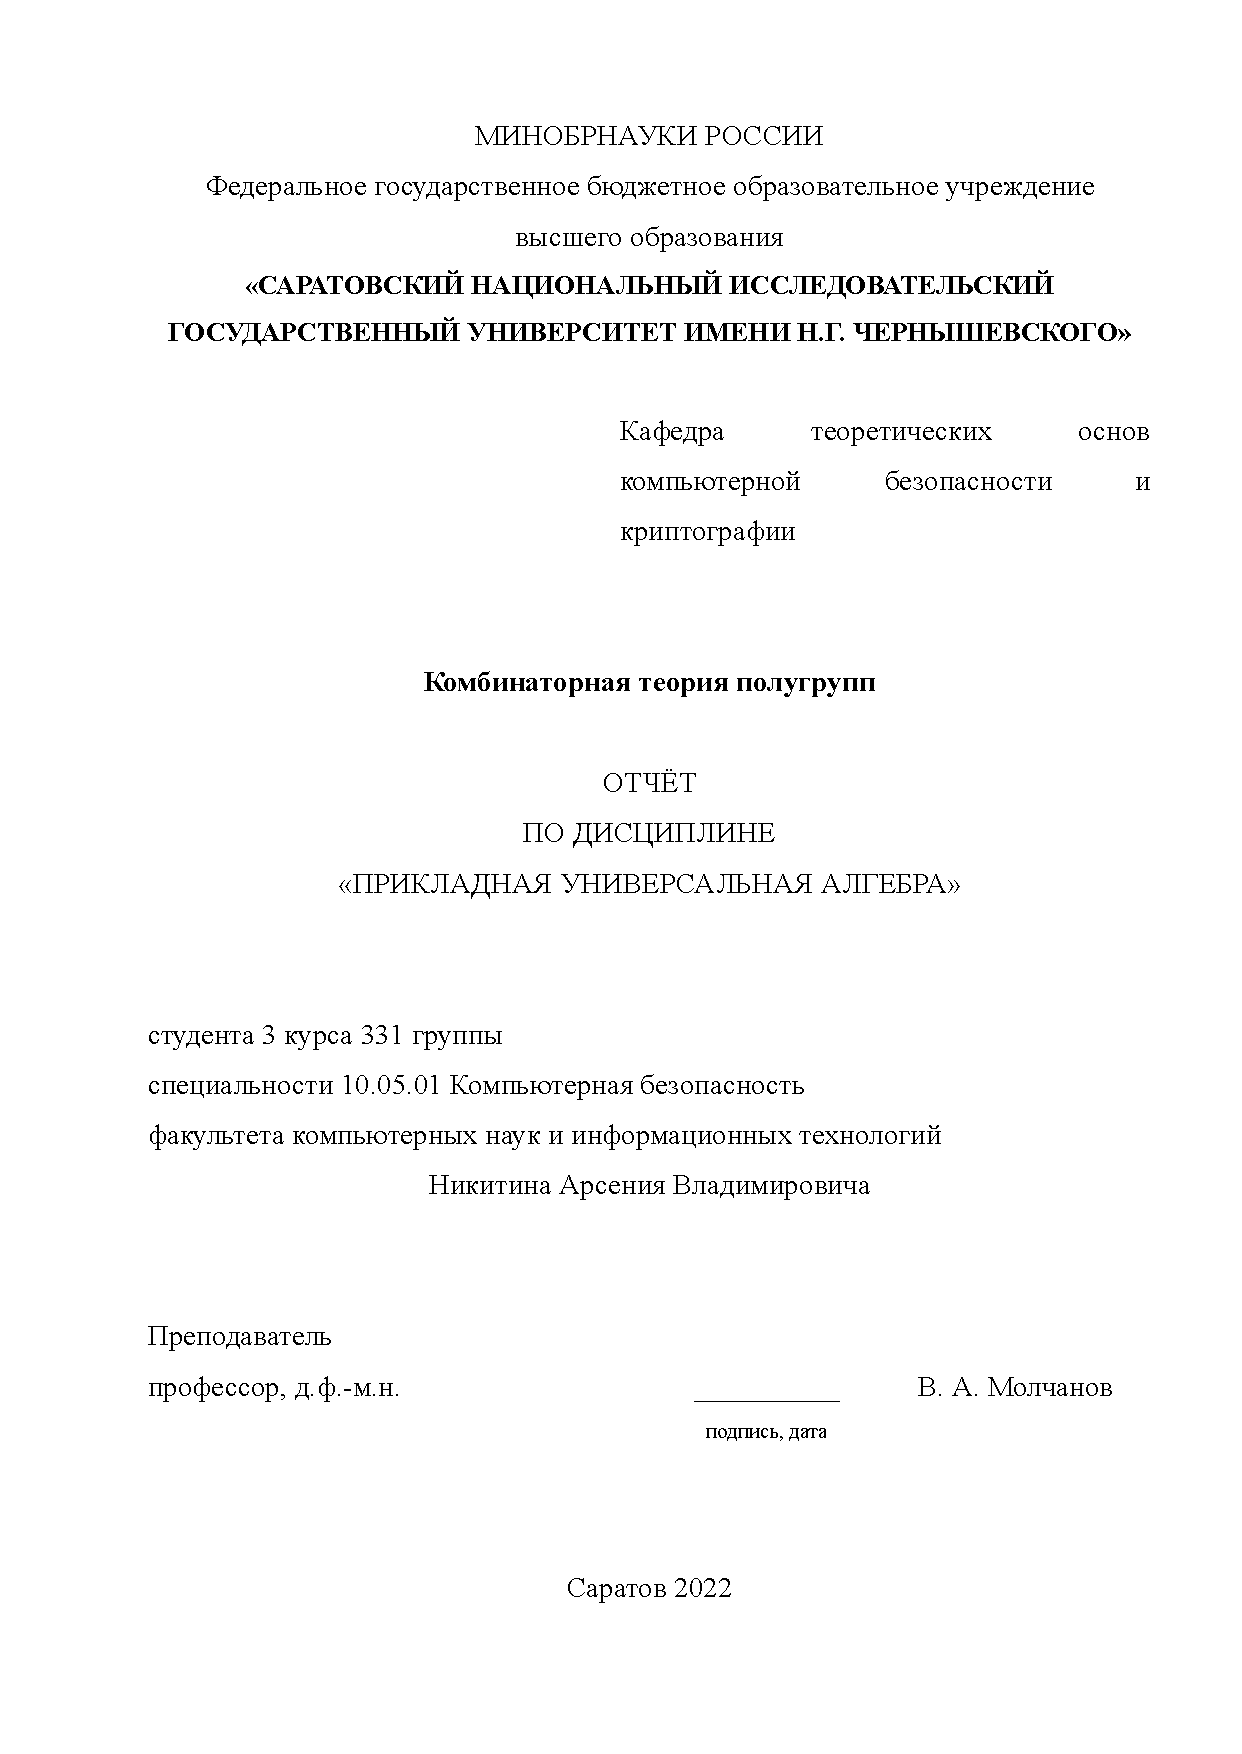
\includepdf{titul.pdf}

%-------------------------------------------------------------------------------

\tableofcontents

\section{\textbf{Цель работы и порядок ее выполнения}}

\textbf{Цель работы} "--- изучение основных понятий теории полугрупп.

Порядок выполнения работы:

\begin{enumerate}
    \item Рассмотреть понятия полугруппы, подполугруппы и порождающего
    множества. Разработать алгоритм построения подполугрупп по таблице Кэли.
    \item Разработать алгоритм построения полугруппы бинарных отношений по
    заданному порождающему множеству.
    \item Рассмотреть понятия подгруппы, порождающего множества и
    определяющих соотношений. Разработать алгоритм построения полугруппы по
    порождающему множеству  и определяющим соотношениям.
\end{enumerate}

\section{Теоретические сведения}


Полугруппа "--- это алгебра $S = (S, \cdot)$ с одной
ассоциативной бинарной операцией $\cdot$, т.е. выполняется $(x \cdot y)
\cdot z = x \cdot (y \cdot z)$ для $\forall x, y, z \in S$. Если
полугрупповая операция называется умножением (или сложением), то полугруппу
называют мультипликативной (или аддитивной).

Подмножество $X$ полугруппы $S$ называется
подполугруппой, если $X$ устойчиво относительно операции умножения, т.е.
$\forall x, y \in X$ выполняется свойство: $x \cdot y \in X$. В этом случае
множество $X$ с ограничением на нем операции умножения исходной полугруппы
$S$ образует полугруппу.

\subsection{Алгоритм построения подполугруппы по заданному порождающему множеству и таблице Кэли}

\textit{Вход} Порождающее множество $S$ длины $n$, подмножество множества $subset$,
таблица Кэли $C = (a_{ij})$ размерности $n \times n$.

\textit{Выход} Подполугруппа $\langle X \rangle \subset S$.

\begin{enumerate}
    \item Создать переменную $x\_current=subset$.
    \item Создать переменную $x\_previous=~'~'$.
    \item Цикл пока $x\_current \not = x\_previous$.
        \begin{enumerate}
            \item Создать пустой список $x\_l$.
            \item Цикл по $i$ от 1 до $|x\_current|$, цикл по $j$ от 1 до $|subset|$.
                \begin{enumerate}
                    \item Создать переменную $x$ и присвоить ей номер позиции
                    $x\_current[i]$ в множестве $S$.
                    \item Создать переменную $y$ и присвоить ей номер позиции
                    $subset[j]$ в множестве $S$.
                    \item Добавить в список $x\_l$ значение $C[x][y]$.
                \end{enumerate}
            \item Присвоить $x\_previous$ значение $x\_current$.
            \item Присвоить $x\_current$ объединение полученных из переменных $x\_l$ 
            и $x\_current$ множеств и сделать из $x\_current$ список.
            \item Отсортировать $x\_current$ по возрастанию.
            \item Если $x\_current = x\_previous$, то ответ --- $x\_current$.
        \end{enumerate}
\end{enumerate}

Трудоемкость алгоритма $O(n^3)$.

В силу общего свойства подалгебр пересечение любого семейства $X_i$ $(i \in I)$ 
подполугрупп полугруппы $S$ является подполугруппой $S$ и, значит, множество $Sub(S)$ 
всех подполугрупп полугруппы $S$ является системой замыканий. множество $X$. Такая 
полугруппа обозначается символом $\langle X \rangle$ и называется подполугруппой 
$S$, порождённой множеством $X$. При этом множество $X$ называется также 
\textbf{порождающим множеством} подполугруппы $\langle X \rangle$. В частности, 
если $\langle X \rangle = S$, то $X$ называется порождающим множеством полугруппы 
$S$ и говорят, что множество $X$ порождает полугруппу $S$.

\subsection{Алгоритм построения полугруппы бинарных отношений по порождающему множеству}

Для реализации алгоритма используется вспомогательный алгоритм\\ $insert\_matrix$,
представляющий из себя добавление в исходное матричное множество матрично перемноженных 
подмножеств множества.

\textit{Вход} Порождающее множество $S$ длины $n$, $k$ матриц бинарных отношений 
$M_k = (m_{k_{ij}})$ размерности $n \times n$.

\textit{Выход} Полугруппа $Sgr$, таблица Кэли $C_{sgr}$ полугруппы $Sgr$.

\begin{enumerate}
    \item Создать пустые отсортированные словари $in\_matrices$ и  $out\_matrices$
    \item Создать переменную $cur=0$.
    \item Создать пустое множество $sets$.
    \item Цикл по $i$ от 1 до $k$.
        \begin{enumerate}
            \item Присвоить $in\_matrices$ по ключу $char(65 + cur)$ значение $M_i$.
            \item Переменной $cur$ присвоить значение $cur+1$.
            \item Присвоить $out\_matrices$ по ключу $M_i$ значение $char(65 + cur)$.
            \item Добавить $M_i$ во множество $sets$.
        \end{enumerate}
    \item Создать множество $group$ и присвоить копию множества $sets$.
    \item Создать переменную $flag$ и присвоить ей значение $True$ (данная переменная
    требуется для того, чтобы была выполнена хотя бы одна итерация следующего цикла).
    \item Создать переменную $cur\_updated=0$
    \item Цикл пока $group \not = sets ~||~ Flag$.
        \begin{enumerate}
            \item Переменной $flag$ присвоить значение $False$.
            \item Цикл по $i$ от 1 до $|sets|$, цикл по $j$ от 1 до $|sets|$.
                \begin{enumerate}
                    \item Создать переменную $new\_matrix$ и присвоить ей умножение
                    матрицы $sets[i]$ на матрицу $sets[j]$ (алгоритм перемножения
                    матриц был рассмотрен в лабораторной работе №1).
                    \item Если $new\_matrix$ не находится в $group$, то:
                        \begin{enumerate}
                            \item Присвоить $in\_matrices$ по ключу $char(65 + cur + cur\_updated)$ 
                            значение $new\_matrix$.
                            \item Переменной $cur\_updated$ присвоить значение $cur\_updated+1$.
                            \item Присвоить $out\_matrices$ по ключу $new\_matrix$ 
                            значение $char(65 + cur + cur\_updated)$.
                            \item Добавить во множество $group$ матрицу $new\_matrix$.
                        \end{enumerate}
                \end{enumerate}
        \end{enumerate}
    \item Если $group = sets$:
        \begin{enumerate}
            \item Полугруппа $Sgr$ получается в результате поиска по ключу в словаре 
            $out\_matrices$, где ключами будут являться элементы множества $sets$.
            \item Множеству $sets$ присвоить значение $insert\_matrix(sets, n)$.
            \item Цикл по $i$ от 1 до $|out\_matrices|$, цикл по $j$ от 1 до $|out\_matrices|$.
                \begin{enumerate}
                    \item Таблица Кэли получается в результате перемножения матриц $in\_matrices$
                    по индексу $char(65 + i)$ и $in\_matrices$ по индексу $char(65 + j)$.
                    Затем происходит поиск значения в словаре $out\_matrices$ по 
                    полученному в результате перемножения матриц ключу. 
                \end{enumerate}
        \end{enumerate}
    \item Ответ --- полугруппа $Sgr$ и ее таблица Кэли $C_{sgr}$.
\end{enumerate}

Трудоемкость алгоритма $O(2^{n^2}n^3)$, так как алгоритм умножения 
матриц имеет трудоемкость $O(n^3)$.\\


Для любой конечной полугруппы $S$ найдется такой конечный алфавит $A$, что для
некоторого отображения $\phi : A \rightarrow S$ выполняется равенство
$\langle \phi(A) \rangle = S$ и, значит, $S \cong A^+/ ker \phi$ этом случае
множество $A$ называется множеством порождающих символов полугруппы $S$
(относительно отображения $\phi : A \rightarrow S$ ). Если при этом для слов
$w_1,w_2 \in A$ выполняется равенство $\phi(w_1) = \phi(w_2)$, т.е. $w_1 \equiv w_2(ker\phi)$, 
то говорят, что на $S$ выполняется соотношение $w_1 = w_2$ (относительно 
отображения $\phi : A \rightarrow S$).

Очевидно, что в общем случае множество таких соотношений $w_1 = w_2$ для всех пар 
$(w_1, w_2) \in ker\phi$ будет бесконечным и не представляется возможности эффективно 
описать полугруппу $S$ в виде полугруппы классов конгруэнции $ker\phi$. Однако в 
некоторых случаях можно выбрать такое сравнительно простое подмножество $\rho \subset ker\phi$ , 
которое однозначно определяет конгруэнцию $ker\phi$ как наименьшую конгруэнцию
полугруппы $A^+$ , содержащую отношение $\rho$, т.е. $ker\phi = f_{con}(\rho) = f_{eq}(f_{reg}(\rho))$.

Так как в случае $(w_1, w_2) \in \rho$ по-прежнему выполняется равенство $\phi(w_1) = \phi(w_2)$, 
то будем писать $w_1 = w_2$ и называть такие выражения \textbf{определяющими соотношениями}. 
Из таких соотношений конгруэнция $ker\phi$ строится с помощью применения следующих процедур к
словам $u,v \in A^+$:


\begin{enumerate}
      \item слово $v$ непосредственно выводится из слова $u$, если $v$
      получается из $u$ заменой некоторого подслова $w_1$ на слово $w_2$,
      удовлетворяющее определяющему соотношению $w_1 = w_2$, т.е. $(u, v) =
      (xw_1y, xw_2y)$ для некоторых $x, y \in A^*$;
      \item слово $v$ выводится из слова $u$, если $v$ получается из $u$ с
      помощью конечного числа применения процедуры $1$.
\end{enumerate}
    
Если все выполняющиеся на $S$ соотношения выводятся из определяющих соотношений 
совокупности $\rho$, то конгруэнция $ker\phi$ полностью определяется отношением 
$\rho$ и выражение $<A: {w_1 = w_2 : (w_1, w_2) \in \rho}>$ называется 
\textbf{копредставлением полугруппы $S$}.


Обозначим символом $A^+$ множество всех непустых слов над алфавитом и символом 
$A^*$ -- множество слов $A^* = A^+ \cup \{\Lambda\}$. На этих множествах слов 
определена операция умножения, которая называется операцией конкатенации слов и 
определяется по правилу: любым словам $w_1 = a_1 \dots a_n$ и $w_2 = b_1 \dots b_m$ 
операция конкатенации ставит в соответствие слово $w_1 \cdot w_2 = a_1 \dots a_n b_1 \dots b_n$. 
В результате множество слов $A^+$ с операцией конкатенации образует полугруппу, 
которая называется полугруппой слов над алфавитом $A$, и множество слов $A^*$ с 
операцией конкатенации образует полугруппу с единичным элементом $\Lambda$, которая
называется моноидом слов над алфавитом $A$.

\subsection{Алгоритм построения полугруппы по порождающему множеству и 
определяющим соотношениям}

\textit{Вход} Элементы алфавита $Alph$ длины $m$, определяющие соотношения $rules$ 
в количестве $n$ штук.

\textit{Выход} Полугруппа и ее таблица Кэли.

\begin{enumerate}
   \item Создать пустое множество $new\_semigroup$.
   \item Создать список $semigroup$ и заполнить его элементами алфавита $Alph$.
   \item Цикл пока $new\_semigroup \not = semigroup$.
        \begin{enumerate}
            \item Создать пустой список $new\_elems$.
            \item Цикл по $i$ от 1 до $|semigroup|$, цикл по $j$ от 1 до $|semigroup|$.
                \begin{enumerate}
                    \item Создать переменную $new\_elem$ и присвоить ей значение 
                    конкатенации слов $semigroup[i] + semigroup[j]$.
                    \item Создать переменную $new\_elem\_copy = ~'~'$
                    \item Цикл пока $new\_elem\_copy \not = new\_elem$.
                        \begin{enumerate}
                            \item Цикл по $key,~value$ из словаря $rules$.
                                \begin{itemize}
                                    \item Если $key$ находится в $new\_elem$, то 
                                    в $new\_elem$ заменить $key$ на $value$. 
                                \end{itemize}
                        \end{enumerate}
                    \item Добавить в список $new\_elems$ строку $new\_elem$.
                \end{enumerate}
            \item Множеству $new\_semigroup$ присвоить копию $semigroup$.
            \item Цикл по $i$ от 1 до $|new\_elems|$.
                \begin{enumerate}
                    \item Если $new\_elems[i]$ не находится в $semigroup$, то
                    добавить \\$new\_elems[i]$ в $semigroup$.
                \end{enumerate}
        \end{enumerate}
    \item Создать пустой список $matrix$.
    \item Цикл по $i$ от 1 до $|semigroup|$.
        \begin{enumerate}
            \item Создать пустой список $matrix\_string$.
            \item Цикл по $j$ от 1 до $|semigroup|$.
                \begin{enumerate}
                    \item Создать переменную $new\_elem=semigroup[i]+semigroup[j]$.
                    \item Создать переменную $new\_elem\_copy=''$.
                    \item Цикл пока $new\_elem\_copy \not = new\_elem$.
                        \begin{enumerate}
                            \item Переменной $new\_elem\_copy$ присвоить копию $new\_elem$.
                            \item Цикл по $key,~value$ из словаря $rules$.
                                \begin{itemize}
                                    \item Если $key$ находится в $new\_elem$, то
                                    заменить в $new\_elem$ $key$ на $value$.
                                \end{itemize}
                        \end{enumerate}
             
                \end{enumerate}
            \item Добавить $new\_elem$ в $matrix\_string$.
        \end{enumerate}
        \item Добавить $matrix\_string$ в список $matrix$.
    \item Ответ --- элементы полугруппы $semigroup$ и таблица Кэли $matrix$ 
    полугруппы $semigroup$.
\end{enumerate}

Трудоемкость алгоритма составляет $O(n^n)$ (процесс построения соотношений 
является бесконечным).


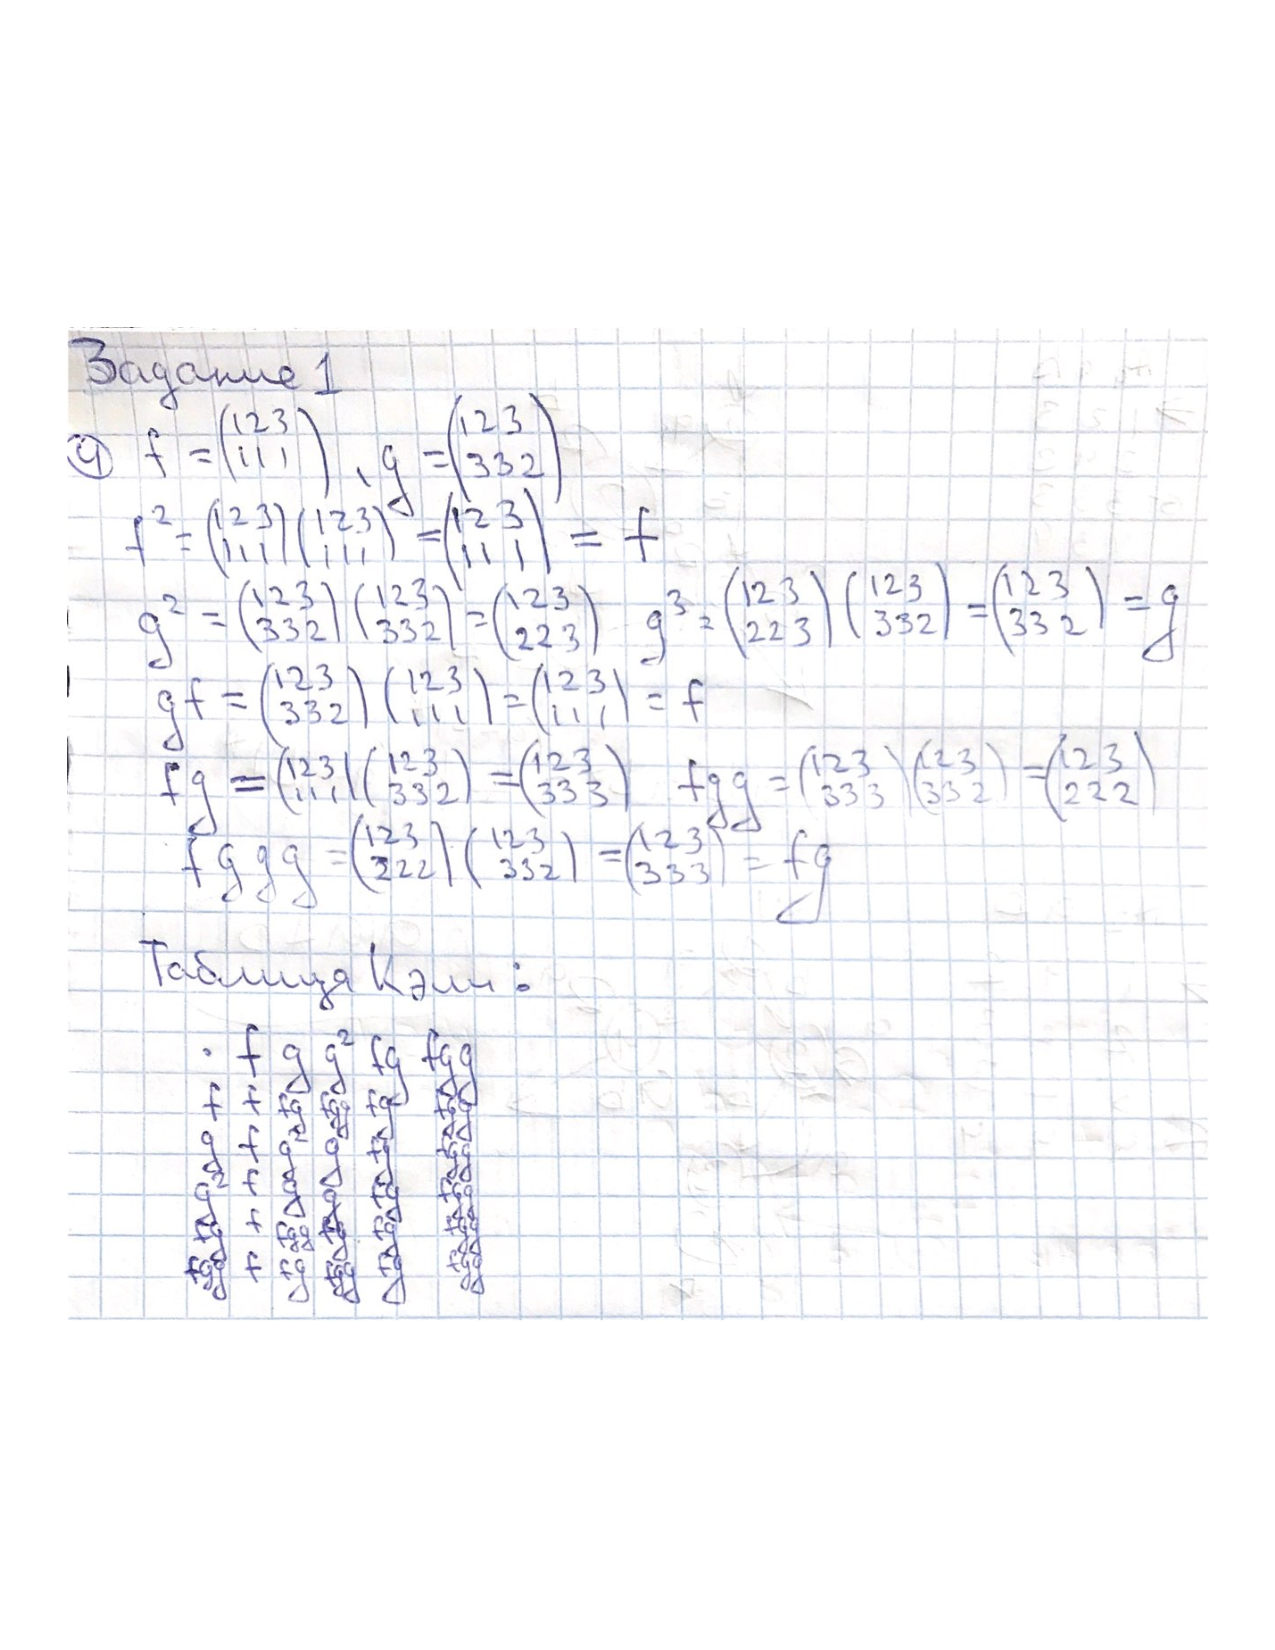
\includepdf[pages={1}, pagecommand=\section{Практическая часть}]{Zad4lab.pdf}
\includepdf[pages={2,3}]{Zad4lab.pdf}\nopagebreak

\begin{table}[h]
    \begin{tabular}{|l|l|l|l|l|l|}
    \hline
    *      & $x$    & $y$    & $y^2$  & $xy$   & $xy^2$ \\ \hline
    $x$    & $y$    & $xy$   & $xy^2$ & $y^2$  & $y$    \\ \hline
    $y$    & $xy$   & $y^2$  & $y$    & $xy^2$ & $xy$   \\ \hline
    $y^2$  & $xy^2$ & $y$    & $y^2$  & $xy$   & $xy^2$ \\ \hline
    $xy$   & $y^2$  & $xy^2$ & $xy$   & $y$    & $y$    \\ \hline
    $xy^2$ & $y$    & $xy$   & $xy^2$ & $y$    & $y$    \\ \hline
    \end{tabular}
    \end{table}

\section{Программная реализация рассмотренных алгоритмов}
    
    \subsection{Результаты тестирования программы}

        \begin{figure}[H]
            \centering
            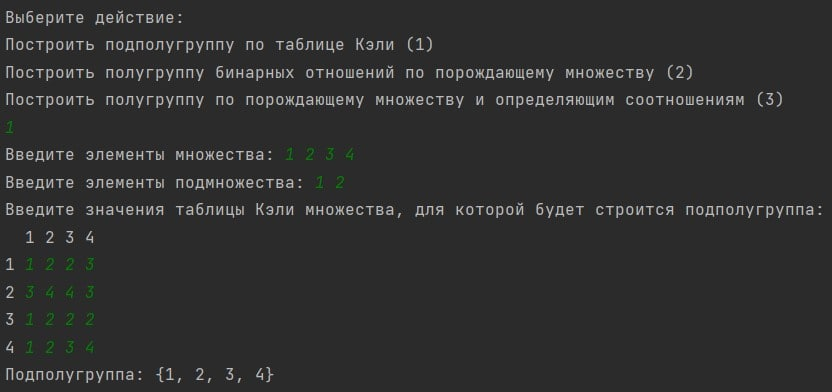
\includegraphics[width=0.8\textwidth]{pic/1.jpg}
            \caption{}
        \end{figure}

        \begin{figure}[H]
            \centering
            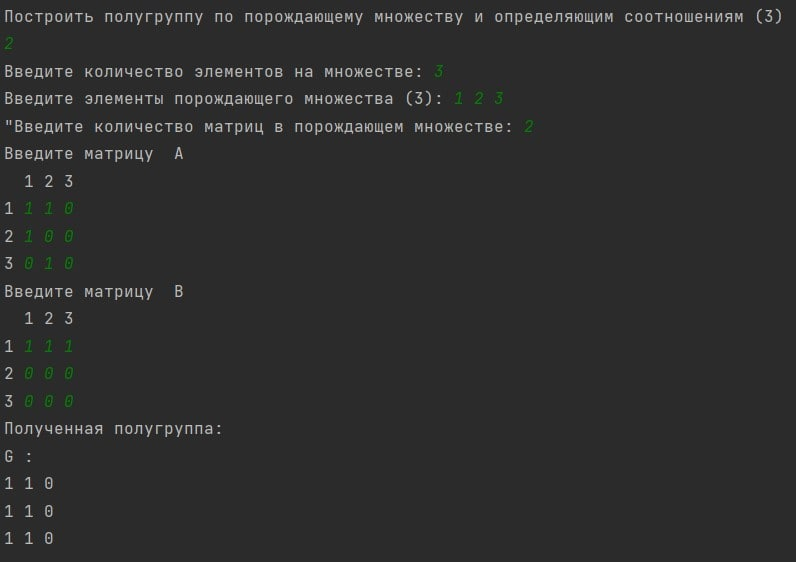
\includegraphics[width=0.8\textwidth]{pic/2.jpg}
            \caption{}
        \end{figure}

        \begin{figure}[H]
            \centering
            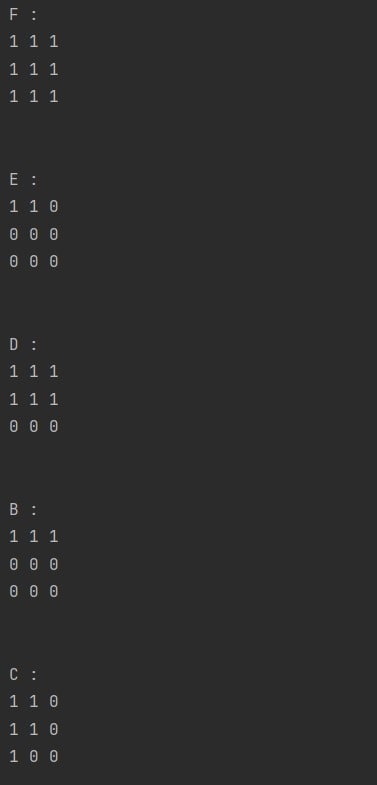
\includegraphics[width=0.8\textwidth]{pic/3.jpg}
            \caption{}
        \end{figure}

        \begin{figure}[H]
            \centering
            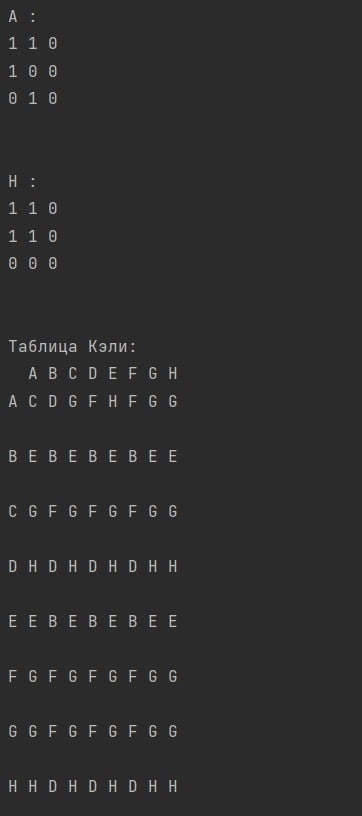
\includegraphics[width=0.8\textwidth]{pic/4.jpg}
            \caption{}
        \end{figure}

        \begin{figure}[H]
            \centering
            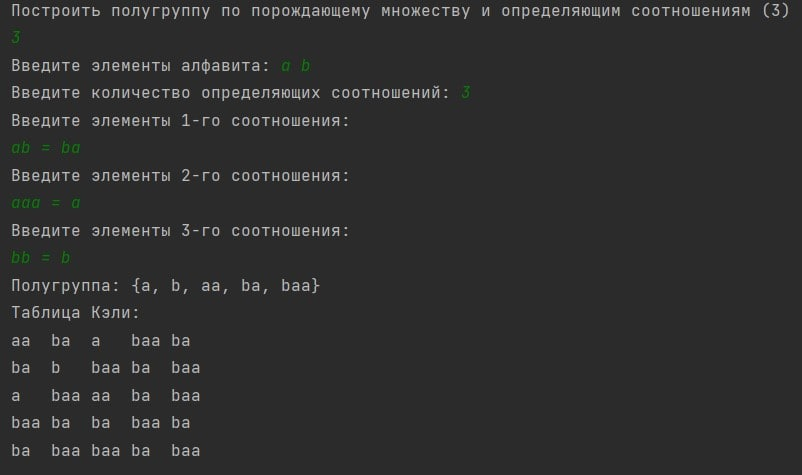
\includegraphics[width=0.8\textwidth]{pic/5.jpg}
            \caption{}
        \end{figure}


        
    \subsection{Коды программ, реализующих рассмотренные алгоритмы}
        \setminted[python]{linenos,breaklines=true, fontsize=\small, style=bw}
        \inputminted{python}{code/lab4.py}
      

\conclusion
В лабораторной работе были рассмотрены теоретические сведения о подгруппах, 
полугруппах, подполугруппах и порождающем множестве. На их основе были составлены 
алгоритмы построения подполугруппы по таблице Кэли, построения полугруппы бинарных 
отношений и ее таблицы Кэли по заданному порождающему множеству, построения 
полугруппы и ее таблицы Кэли по порождающему множеству и определяющим соотношениям. 
Для всех алгоритмов была произведена оценка трудоемкости. 

\end{document}